\chapter{Applications to Elliptic Curves}

In this final chapter, we analyse the case of elliptic curves, consider the technique of uniformization and contrast it to the approaches we have seen so far.

\section{Non-Archimedean Uniformization}

Assume $k$ is algebraically closed.
Let $X$ be the $R$-curve given by the equation $xyz + \pi(x^3 + y^3 + z^3).$
Then, $\hat{X}$ is a formal model for $\anl X_k$ and can be used to give an explicit picture of the latter.

Firstly, the special fiber is given by the vanishing of the function $xyz$, where $x, y, z$ are considered as coordinates on $\mathbb{P}^2_{\tilde{k}}$.
Hence, the special fiber $\hat{X}_s$ is a `cycle of projective lines.'
Although $\anl{X_k}$ may be explicitly determined without much difficulty in this case by gluing, we may more immediately determine its geometry using \cref{boshlutkebohmert}.
Each irreducible component gives a type II point contained in the semistable vertex set.
The ordinary double points have formal fiber given by an open annulus while the smooth, closed points of each affine line correspond to an open ball.
Note that the smooth closed points, and hence the open balls which retract to each type II point in the semistable vertex set, are in bijection with the set $\mathbb{P}^{1, \operatorname{an}}_{\tilde{k}} \backslash \{0, \infty \}$.
This gives the semistable decomposition; the associated skeleton is a triangle.
We obtain the explicit picture shown in \cref{fig:ellipticcurve}.

Speaking more generally, the curve $X_k$ defines an elliptic curve over $k$ with multiplicative reduction.
When working over $\CC$, the uniformization theorem states that any elliptic curve defined over $\CC$ is analytically isomorphic to a quotient $\CC/\Lambda$ by a lattice $\Lambda$ \parencite[\S VI.5]{silverman}.
To find an analog when working over non-Archimedean fields, Tate observed that changing variables using the map $z \mapsto \exp{(2 \pi i z)}$ gives an isomorphism $\CC/\Lambda \to \CC^{\times}/q^{\ZZ}$, where $q = \exp{(2 \pi i \zeta)}$.
Although $\mathbb{Q}_p$ has no non-trivial discrete subgroups, the multiplicative group $\mathbb{Q}_p^{\times}$ does, and this observation spurred the development of rigid analytic spaces and $p$-adic uniformization theory.

In the Berkovich setting, we let $E$ be an elliptic curve over $k$ with multiplicative reduction, in which case $E$ is known as a \textit{Tate curve}.
Then, there exists some $q \in k^{\times}$ with $\zeta = |q| < 1$ such that $\anl{E}$ is formed from the closed annulus $\berkspeck{t, \zeta t^{-1}}$ by gluing along the isomorphism of affinoid domains $\berkspeck{\zeta^{-1} t, \zeta t^{-1}} \cong \berkspeck{t, t^{-1}}$.
The claim is that there exists an isomorphism of $k$-analytic spaces \[\anl{E} \cong \torusan/q^{\ZZ}.\]

If $a \in k^{\times}$ is any element, then it induces an automorphism of $\mathbb{P}^{1}_{k}$ by multiplication by $a$.
This extends to an automorphism $\gamma_a$ of $\projlinean$ by mapping a point $x \in \projlinean \backslash \projlinean(k)$ to the point $a \cdot x$ given by $|f(t)|_{a \cdot x} = |f(a \cdot t)|_x$, for any $f(t) \in k[t]$ \parencite[\S II1.3]{uniformization2}.
It is worth determining more concretely the effect of this action.
Denote $\xi = |a|$ and for each $n \in \ZZ$, denote $A_n = \berkspec{k\{ \xi^{-(n - 1)} t, \xi^{n} t^{-1}\}}$ for some $n \in \ZZ$.
Then $a \cdot x$ is such that $|t|_{a \cdot x} = |a| \cdot |t|_x = \xi \cdot |T|_x$, which shows that $a \in A_{n + 1}$.
Since there is an inverse automorphism induced by multiplication by $a^{-1}$, it follows that $\gamma_a$ defines a map $A_n \to A_{n + 1}$.
In fact, this map is an isomorphism induced by the isomorphism of $k$-affinoid algebras
\begin{align*}
    k\{\xi^{-n} t, \xi^{n + 1} t^{-1} \} & \to k\{\xi^{-(n - 1)} t, \xi^{n} t^{-1} \} \\
    \sum_{m = -\infty}^{\infty} c_{m} t^{m} & \mapsto \sum_{m = -\infty}^{\infty} c_{m} a^m t^{m}
\end{align*}
We have that $\torusan = \bigcup A_{n}$, so that $\gamma_a$ restricts to an automorphism of $\torusan$.
Now, letting $a = q$ and $\Gamma = q^{\ZZ}$ be the infinite cyclic subgroup of $k^{\times}$ generated by $q$, we see that $\Gamma$ has an action on $\torusan$.
This action is properly discontinuous, since for each point we may take an open neighbourhood $U$ isomorphic to an open annulus $\mathbb{S}(q')$, where $|q'| < |q|$, and it follows that $\gamma_{q^m}(U) \cap U$ is empty for any $m \neq 0$.
It follows similarly to the complex analytic case that we may form a $k$-analytic space $\torusan/q^{\ZZ}$, and our description of the action of $q$ on $\torusan$ coupled with the construction of $\torusan/q^{\ZZ}$ then shows that $\anl{E} \cong \torusan/q^{\ZZ}$.

The theory of semistable vertex sets may be applied to the Tate curve.
Let $p = \sqrt{q}$ and $\xi = |p| = \zeta^{1/2}$, and observe that $\anl{E}$ can equivalently be described by gluing the annuli $\berkspeck{t, \xi t^{-1}}$ and $\berkspeck{\xi^{-2} t, \xi t^{-1}}$ appropriately.
The points with representatives $\zeta_{0, 1}$ and $\zeta_{0, \xi}$ then form a semistable vertex set $V$, and the corresponding skeleton $\Sigma(\anl{E}, V)$ is topologically a circle.

We also remark that the isomorphism $\anl{E} \cong \torusan/q^{\ZZ}$ may be used to determine a skeleton for $\anl{E}$.
Recall that there exists a closed subset of $\torusan$ which is homeomorphic to $\mathbb{R}_{> 0}$ by the map $r \mapsto \zeta_{0, r}$, and such that $\torusan$ deformation retracts onto this subspace. 
Now, the action of $q$ on this subspace has the effect of identifying a point $\zeta_{0, r}$ with $\zeta_{0, |q|\cdot r}$, resulting in the same skeleton as we obtained using the approach of semistable vertex sets.

\begin{figure}[!ht]
    \centering
    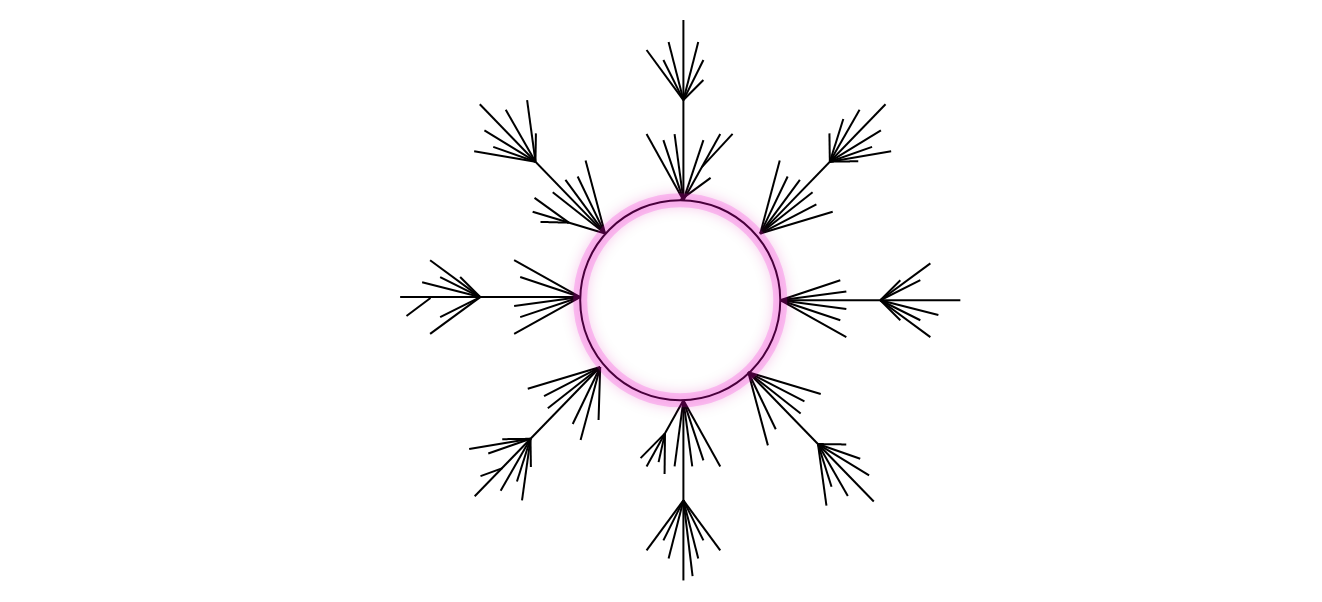
\includegraphics[width=1.0\textwidth]{Images/ellipticcurve.png}
    \caption{A visualisation of the analytification of an elliptic curve with multiplicative reduction.
    The skeleton, which is highlighted here, is a circle.}
    \label{fig:ellipticcurve}
\end{figure}

\section{SNC Models for Elliptic Curves}

\begin{figure}[!ht]
    \centering
    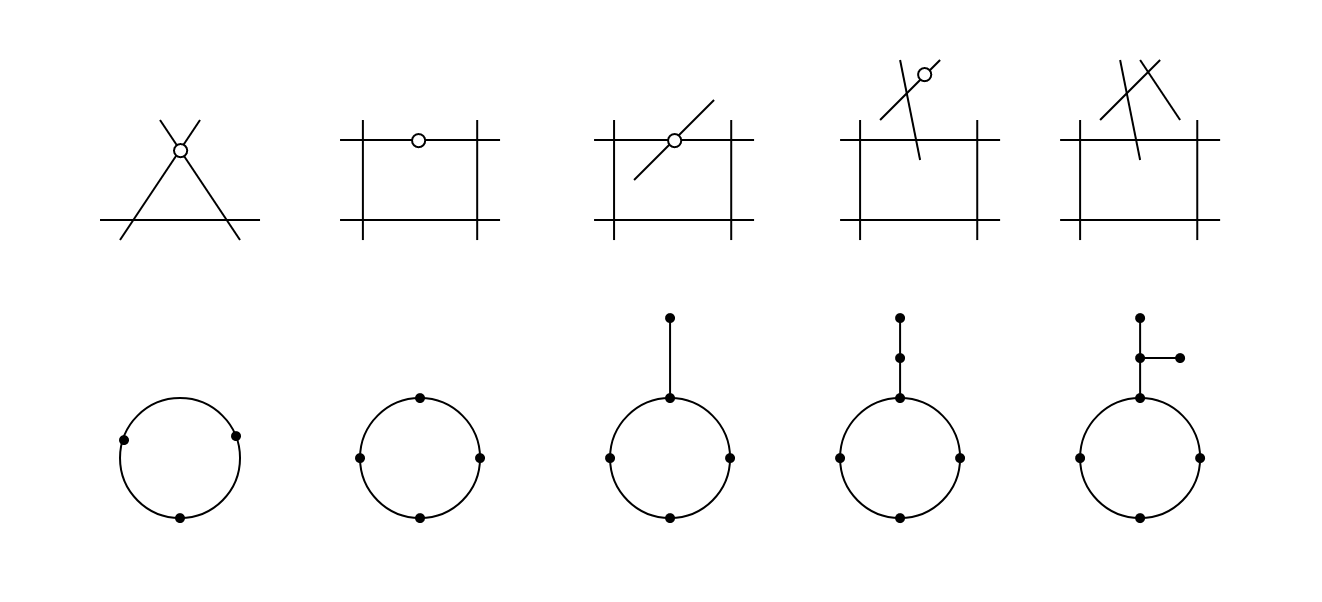
\includegraphics[width=1.0\textwidth]{Images/projectivelimit.png}
    \caption{Diagram indicating how a sequence of point blow-ups of the special fiber affects the skeleton.
    The top row depicts the special fibers of each model, with the next model obtained by a blow-up with the center indicated by a circle.
    The bottom row depicts the dual complex.}
    \label{sequenceofpointblowups}
\end{figure}

We may also consider how the theory of snc models may be used to determine the geometry of the analytification of an elliptic curve $E$ with multiplicative reduction when working over a discrete valuation ring.
In this case, $E$ admits a proper regular model $\model$ over $R$ and
Tate's algorithm may then be used to compute the structure of the special fiber $\model_s$ \parencite[\S IV.9, Theorem 8.2]{silverman}.
Informally, $\model_s$ consists of $n$ rational curves, each appearing with multiplicity one, arranged in the shape of an $n$-gon for some $n \geq 1$.
We assume that $n \geq 2$; then, in such an arrangement, each intersection is transversal, and in particular $\model$ is an snc model for $E$.
The dual graph is then also given by an $n$-gon, hence, it is homeomorphic to a circle once more.
We may recover the full picture of $\anl{E}$ by taking sequences of blow-ups and passing to the projective limit.
This procedure is depicted for $n = 3$ in \cref{sequenceofpointblowups}.
In the general case, we obtain a picture similar to \cref{fig:ellipticcurve}.

A benefit of working with snc models is that we may also investigate the topology of elliptic curves other than those with multiplicative reduction.
We remark that in the case where the elliptic curve $E$ has good reduction, Tate's algorithm indicates that there exists a proper regular model $\model$ where $\model_s$ consists of a single non-singular curve. 
In this case, the dual graph consists of a point, indicating that the space $\anl{E}$ is contractible.
